% \section{Benchmark Design}
% \section{Model Workloads and Target Operators}
\section{\system-Bench}
\label{sec:workloads}
% \ahan{We cannot directly talk about our benchmark. There needs to be sufficient buildup and motivation. We need to motivate why our benchmark is necessary: i.e. what does it plug in the existing literature that other benchmarks do not consider?}\wangjia{done.}

\minjia{Please restructure Section 4 as ADopt-Bench. The current section reads more like workload preparation for our experiments than an independent benchmark contribution. Please look at the intro to see how ADopt-bench is introduced and its position in the paer. We should explain what makes ADopt-Bench different from existing kernel benchmarks, and how each task incorporates its training and deployment context. Make the task specification, model and operator coverage, submission interface, and assessment protocols explicit. A reader should understand how to use ADopt-Bench to evaluate their own kernel agents without relying on ADopt's seed synthesizer or evolver. 1-1.5 pages.}

We prepare primitive and composite kernel targets together with model-training workloads to instantiate $\mathcal I=(\mathcal O,M,W)$. The operators define the kernel-optimization tasks; each model and its declared training setup provide the context for model-level verification and evaluation. Two principles guide preparation: training kernels are assessed as forward--backward implementations, and their configurations come from the workloads in which they are deployed. Calls recorded from source models running on real datasets support operator verification and timing. Candidates are assessed through their autograd interfaces and, where supported, within those models. Figure~\ref{fig:workload_overview} summarizes the prepared workload categories. We next describe the target operators, workload-derived configurations, and experimental selections.

\begin{figure}[h]
    \centering
    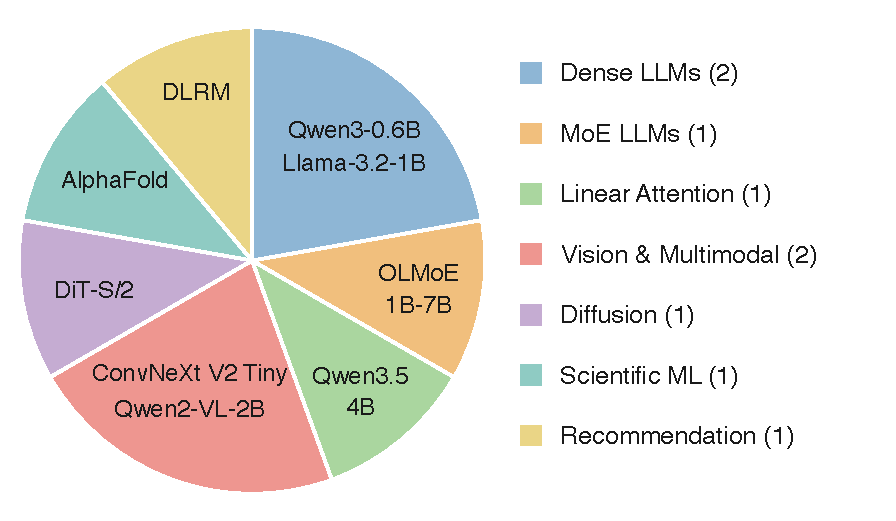
\includegraphics[width=\linewidth]{figures/benchmark_overview.pdf}
    \caption{Prepared models across seven workload categories. Numbers indicate the number of model workloads in each category. }
    \label{fig:workload_overview}
\end{figure}

% \noindent\textbf{Performance and saved memory.} 
% \bench measures execution time and the logical size of tensors retained in $s_p$ for backward to characterize compute--memory tradeoffs. Whole-model evaluation also reports peak allocated GPU memory. Section~\ref{sec:evaluation_protocol} defines the measurement scopes, speedups, and memory accounting.

% \subsection{Model-Driven Benchmark Construction}
\subsection{Target Operators and Workload Preparation}
\label{sec:target_preparation}
\label{sec:workload_configs}
For our experiments, we select kernel targets from prepared model-training workloads. Starting from a source model, we identify computations that form meaningful kernel-optimization boundaries and record their model sites for verification and evaluation. For each source model, we fix the training workload and extract tensor shapes, dtypes, memory layouts, and static operator parameters from forward--backward execution. Calls sharing the same reference computation and configuration form one kernel task, whose manifest records model locations and call counts so that repeated calls across layers do not create duplicate tasks. These targets comprise primitive and composite operators.

\noindent\textbf{Primitive operators.}
Primitive targets include reusable computations such as normalization, activation, reduction, loss, matrix multiplication, convolution, positional encoding, and attention. Each task specifies a PyTorch forward computation and its required gradients, evaluating the generation and optimization of a single autograd-compatible operator.

\noindent\textbf{Composite operators.}
Composite targets group adjacent computations that form a meaningful optimization target in a model's training path, such as linear projection followed by activation, residual addition followed by normalization, or attention computations that span multiple primitive operations. These tasks expose optimization opportunities across operator boundaries, including fusion, elimination of intermediate global-memory traffic, and joint forward--backward implementation choices.
% We use the term \emph{composite operator} rather than \emph{fused operator}: the benchmark defines the computation that must be implemented, while fusion remains an implementation choice available to the system being evaluated.

\noindent\textbf{Training execution.}
Each workload specifies complete model-training execution, including forward computation, loss computation, backward propagation, optimizer update, and gradient reset. Supported optimized implementations are installed at their corresponding operator boundaries throughout the model, where they execute alongside the remaining model computation and framework overhead. Model-scope evaluation measures their effect on end-to-end training time and peak allocated GPU memory.

Primitive and composite targets expose the computations available for kernel synthesis and evolution. The supplied model workload provides the context for deployment verification and measurement of training time and memory. The system returns optimized kernel implementations with their deployment bindings.

% \subsection{Workload-Driven Configurations}
% \label{sec:benchmark_workloads}
% We instantiate the tasks of each source model top-down from an explicitly specified training workload. Standalone operator benchmarks, such as those in Liger-Kernel~\cite{hsu2024liger}, evaluate kernels over predefined shape sweeps; our tasks additionally retain their source-model and training contexts. For each source model, we fix the architecture, batch size, input extent, data type, and execution backend, which determine the operator configurations, and the training data used by the workload (Table~\ref{tab:benchmark_composition}).

% \noindent\textbf{Configuration extraction.}
% We execute a forward--backward pass and record tensor shapes, dtypes, memory layouts, and static operator parameters at the Level~1--2 boundaries defined in Section~\ref{sec:benchmark-hierarchy}. Calls to the same reference computation under equivalent configurations form one task; different configurations form separate tasks. The workload manifest records each task's source model, workload settings, model locations, and call count, so repeated calls across layers increase its frequency without creating duplicate tasks.


\subsection{Prepared Workloads and Target Configurations}
\label{sec:workload_composition}

Table~\ref{tab:workload_composition} summarizes the prepared source models, workload data, precision settings, and available primitive/composite configurations. Section~\ref{sec:results} reports a subset of these workloads and targets. Detailed configurations and experimental selections appear in \appref{app:operator_configs}.

\begin{table}[t]
\centering
\caption{Prepared model workloads and operator configurations. P and C count primitive and composite configurations; M counts model workloads. Mixed denotes FP32 with BF16 autocast.}
\label{tab:workload_composition}
\begingroup
\small
\setlength{\tabcolsep}{3pt}
\renewcommand{\arraystretch}{1.05}
\begin{tabularx}{\columnwidth}{@{}Xlcrrr@{}}
\toprule
\textbf{Model}
& \textbf{Workload data}
& \textbf{dtype}
& \textbf{P}
& \textbf{C}
& \textbf{M} \\
\midrule

\multicolumn{6}{@{}l}{\emph{Dense LLMs}} \\
Qwen3-0.6B & WikiText-2 & BF16 & 14 & 4 & 1 \\
Llama-3.2-1B & WikiText-2 & BF16 & 11 & 4 & 1 \\

\multicolumn{6}{@{}l}{\emph{MoE LLMs}} \\
OLMoE-1B-7B & WikiText-2 & BF16 & 8 & 4 & 1 \\

\multicolumn{6}{@{}l}{\emph{Linear attention}} \\
Qwen3.5-4B & WikiText-2 & BF16 & 20 & 7 & 1 \\

\multicolumn{6}{@{}l}{\emph{Vision and multimodal}} \\
ConvNeXt V2-Tiny & Imagenette & BF16 & 31 & 4 & 1 \\
Qwen2-VL-2B & TextVQA & BF16 & 16 & 2 & 1 \\

\multicolumn{6}{@{}l}{\emph{Diffusion}} \\
DiT-S/2 & Imagenette & FP32 & 10 & 2 & 1 \\

\multicolumn{6}{@{}l}{\emph{Scientific ML}} \\
MegaFold (AF3) & PDB & Mixed & 2 & 2 & 1 \\

\multicolumn{6}{@{}l}{\emph{Recommendation}} \\
DLRM & Criteo Kaggle & FP32 & 7 & 1 & 1 \\

\midrule
\textbf{Total} & & & \textbf{119} & \textbf{30} & \textbf{9} \\
\bottomrule
\end{tabularx}
\endgroup
\end{table}

These model-derived tasks connect the framework's implementation search to the training contexts in which its outputs are assessed. Section~\ref{sec:results} evaluates a subset of 18 primitive cases, 17 composite cases, and six prepared model workloads.
